\documentclass[25pt, a0paper, portrait, blockverticalspace=.5cm]{tikzposter}
\usepackage[utf8]{inputenc}
\usepackage{amssymb,amsfonts,amsmath,mathtext,mathtools}
\usepackage{xfrac}
\usepackage{enumitem}

\usepackage{makecell}
\usepackage{amsmath}

\let\vec\oldvec
\newcommand{\vec}[1]{\boldsymbol{#1}}

\title{\parbox{\linewidth}
	{\centering
		Spin coherence and betatron chromaticity of deuteron beam in NICA storage ring\\		
}}

\author{S. Kolokolchikov\textsuperscript{1}*, Y. Senichev\textsuperscript{2}, \\A. Aksentyev\textsuperscript{2}, A. Melnikov\textsuperscript{2}}
\institute{
	\textsuperscript{1} International Union of Pure and Applied Physics, Geneva, Switzerland\\
	\textsuperscript{2} Institute for Nuclear Research of the Russian Academy of Sciences, Moscow, Russia\\
	*sergey.bell13@gmail.com
}
\usetheme{Simple}
\usecolorstyle{Russia}
\colorlet{blocktitlefgcolor}{black}

\usepackage{caption}
\captionsetup{font=large}
\usepackage{multicol}
\setlength\columnsep{1.5cm}

\begin{document}

\maketitle


\begin{columns}
\column{.33}

\block{INTRODUCTION}{

\par For \textbf{Electric Dipole Moment} (EDM) the possibility of spin control experiment can be done by setting Wien Filters in straight ByPass sections, which ensure that the particles spin retains mean direction in accordance with~"Quasi-Frozen~Spin"~mode.
However, the spin of different particles, due to their different motion in 3D space, in any case rotates with
slightly different frequencies around the invariant axis, which one violates spin coherence. To ensure spin
coherence, nonlinear elements, sextupoles, with a special placement on arcs must be used. Since sextupoles
simultaneously affect the betatron chromaticity, we consider this complicated case.
}

\block{EDM SEARCH}{

\par T-BMT equations describe the evolution of $\vec{S}$ – spin-vector over time in particle rest frame in $\vec{E}, \vec{B}$ fields in laboratory frame:

\begin{equation}\label{eq:T-BMT}
\begin{aligned}
\frac{{d \vec{S}}}{d t} &=\vec{S} \times\left(\vec{\Omega}_{MDM}+\vec{\Omega}_{EDM}\right), \\
\vec{\Omega}_{MDM}&=\frac{q}{m \gamma}\left\{(\gamma G+1)\vec{B}_{\perp}+(G+1)\vec{B}_{\parallel}-\right. \\
&\left.-\left(\gamma G+\frac{\gamma}{\gamma+1}\right) \frac{\vec{\beta} \times \vec{E}}{c}\right\}, \\
\vec{\Omega}_{EDM}&=\frac{q \eta}{2 m}\left(\vec{\beta} \times \vec{B}+\frac{\vec{E}}{c}\right), \quad G=\frac{g-2}{2},
\end{aligned} 
\end{equation}

\par It is necessary to lower the impaction from MDM. But NICA has purely magnetic arcs. Thus, it can not be used "Frozen Spin" Method [1]. Wien Filters implemented in the straight section compensate rotation via MDM in arc and realise a "Quasi-Frozen Spin" condition for deutrons [2]. For this needs NICA needs a modernisation to use NICA as storage ring with alternative straight sections by using ByPass channels [3].

}	

\block{SPIN TUNE DECOHERENCE}{
\par If we follow T-BMT equations, spin-tunes in $E, B$ fields are given by the expressions:

\begin{equation}\label{eq:spintune}
\begin{aligned}
v_s^B & =\gamma G, \\
v_s^E & = \frac{G+1}{\gamma}-G \gamma .
\end{aligned}
\end{equation}

\section*{An Equilibrium Level Energy Shift}

\par Because different particles move with various energy, there is a need to use effective energy:

\par \begin{equation}\label{eq:gamma_eff}
\gamma_{eff} = \gamma_{s}+\beta_{s}^2 \gamma_{s} \Delta \delta_{e q}
\end{equation}

\par The equilibrium momentum spread due to the betatron motion and non-zero second order momentum compaction factor based on synchronous acceleration principle \cite{Decoherence} and is given:

\begin{equation}\label{eq:delta_eq}
\Delta \delta_{e q}=\frac{\gamma_s^2}{\gamma_s^2 \alpha_0-1}\left[\frac{\delta_0^2}{2}\left(\alpha_1+\frac{3}{2} \frac{\beta_s^2}{\gamma_s^2}-\frac{\alpha_0}{\gamma_s^2}+\frac{1}{\gamma_s^4}\right)+\left(\frac{\Delta L}{L}\right)_\beta\right],
\end{equation}

\section*{Orbit Lengthening}

\par More formal theory implies the interaction of external (sextupole) field. Taking into account the expression for total orbit lengthening from \cite{Lengthening}:

\begin{equation}\label{eq:delta_C}
\Delta C_{\Sigma}=- \pi\left(\varepsilon_x \xi_x+ \varepsilon_y \xi_y\right)+\delta_0\left(\alpha_0+\alpha_1 \delta_0+\ldots\right),
\end{equation}
}

\column{.66}

\block{SEXTUPOLE CORRECTION}{
		\begin{minipage}{0.5\linewidth}
			\begin{tikzpicture}
			\node (cone) at (0,0) {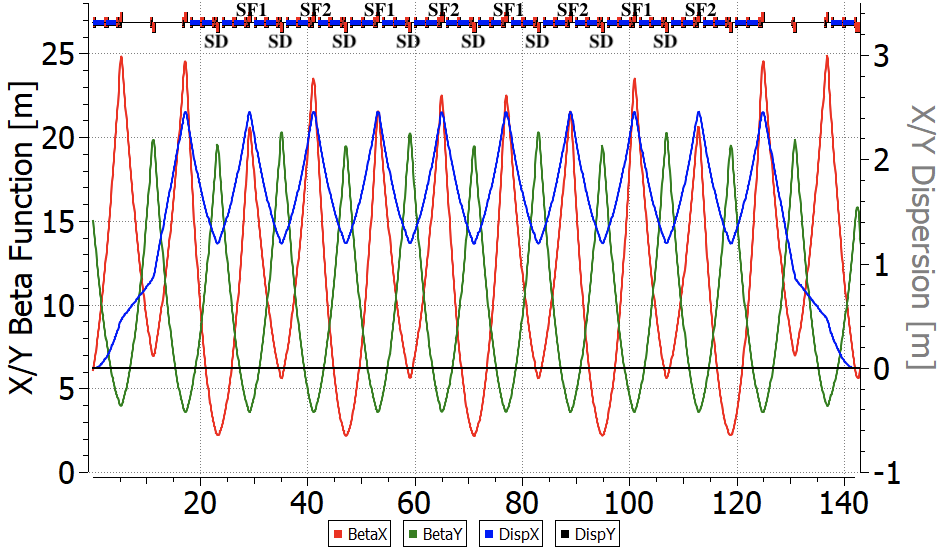
\includegraphics[width=\linewidth]{TEXPaper/img/MOPA070_f1-1.png}};
			\end{tikzpicture}
		\end{minipage}
		\begin{minipage}{0.05\linewidth}
		\par  $.$
		\end{minipage}
		\begin{minipage}{0.45\linewidth}
		\par As a result Eqs.~\ref{eq:delta_eq}, \ref{eq:delta_C} show that using sextupoles can influence $\Delta\nu_{s}$ and allow to get 		spin coherence.
		\par 	Sextupoles can influence only if they located in non-zero dispersion regions. In minimum/maximum of dispersion $D_{x, y}$ 		and  beta $\beta_{x, y}$ functions for the most impact. Dispersion is suppressed with missing magnets at the edges.
		Shown Twiss-functions in OptiM of ByPass NICA arc for deuteron mode. Also shown sextupole families arrangement.
		\end{minipage}
		\newline
		\newline
		
		
		\begin{minipage}{0.235\linewidth}
			\begin{tikzpicture}
			\node (cone) at (0,0) {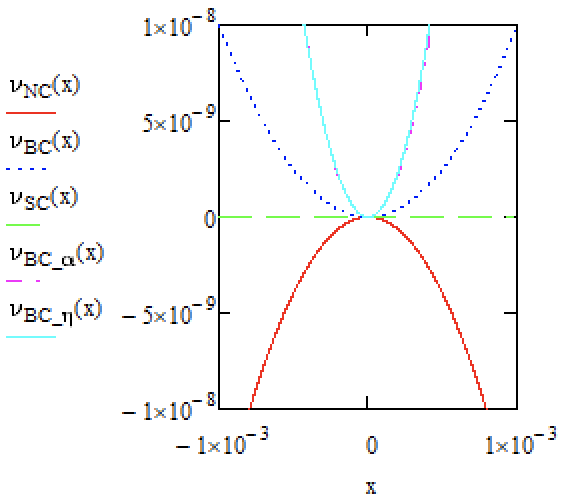
\includegraphics[width=\linewidth]{TEXPaper/img/MOPA070_f2-1.png}};
			\end{tikzpicture}
		\end{minipage}
		\begin{minipage}{0.235\linewidth}
			\begin{tikzpicture}
			\node (cone) at (0,0) {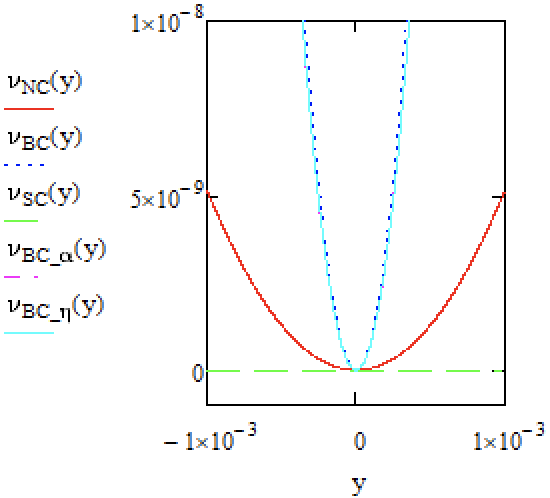
\includegraphics[width=\linewidth]{TEXPaper/img/MOPA070_f2-2.png}};
			\end{tikzpicture}
		\end{minipage}
		\begin{minipage}{0.235\linewidth}
			\begin{tikzpicture}
			\node (cone) at (0,0) {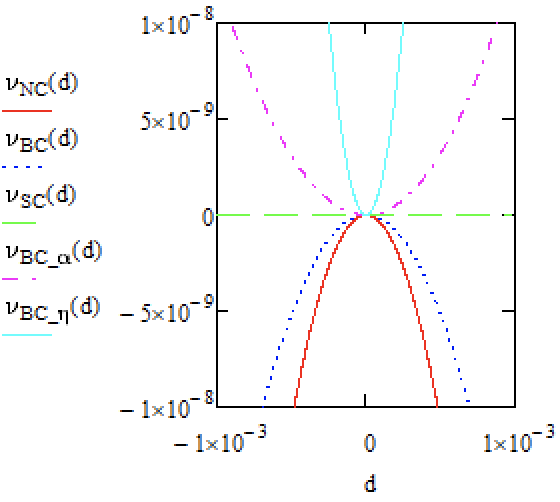
\includegraphics[width=\linewidth]{TEXPaper/img/MOPA070_f2-3.png}};
			\end{tikzpicture}
		\end{minipage}
		\begin{minipage}{0.04\linewidth}
		\par  $.$
		\end{minipage}
		\begin{minipage}{0.235\linewidth}
		\par Spin-tune dependance on x, y, d for various cases. NC – natural chromaticity (red); BC – zero chromaticity (blue dotted); SC – spin coherence (green); BC$\underline {\hspace{0.2cm}}$$\alpha$ –  zero chromaticity and zero $\alpha_{1}$ (violet); BC$\underline {\hspace{0.2cm}}$$\eta$ –  zero chromaticity and zero $\eta_{1}$ (light blue).
		\end{minipage}
		\newline
		\newline
		
		\begin{minipage}{0.3\linewidth}
		 	\section*{Betatron Chromaticity}
			\begin{tikzpicture}
			\node (cone) at (0,0) {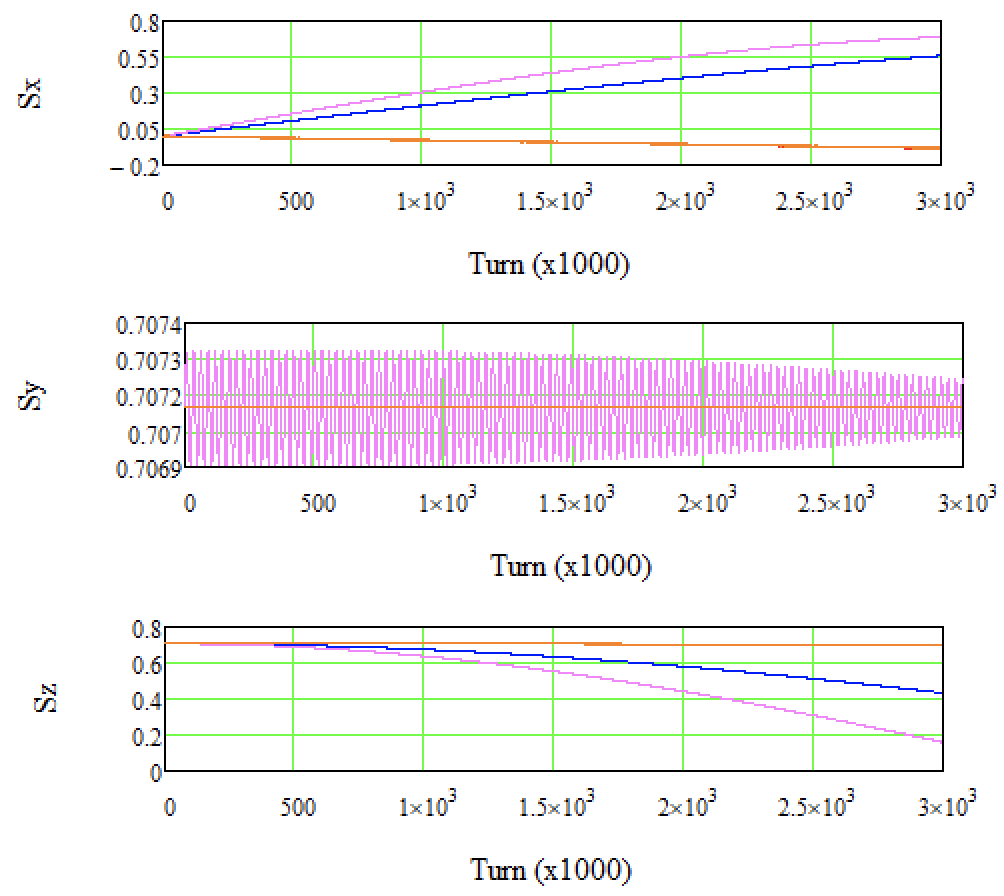
\includegraphics[width=\linewidth]{TEXPaper/img/MOPA070_f3-1.png}};
			\end{tikzpicture}
			\par Spin Tracking for particles with various initial deviation in $x, y, d$ – coordinates using 2 sextupole families 					to get zero chromaticity.
		\end{minipage}
		\begin{minipage}{0.05\linewidth}
		\par  $.$
		\end{minipage}
		\begin{minipage}{0.3\linewidth}
			\section*{Spin Coherence}
			\begin{tikzpicture}
			\node (cone) at (0,0) {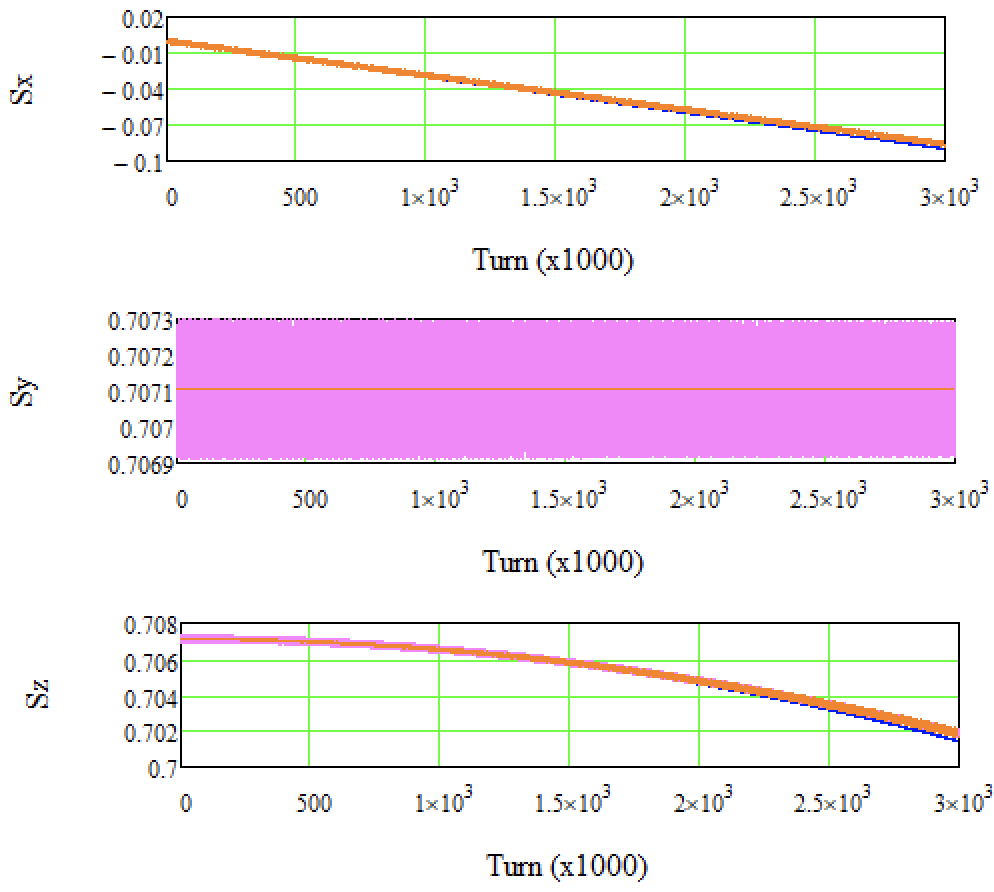
\includegraphics[width=\linewidth]{TEXPaper/img/MOPA070_f4-1.png}};
			\end{tikzpicture}
			\par Spin Tracking for particles with various initial deviation in $x, y, d$ – 
			coordinates using 3 sextupole families to get spin coherence.
		\end{minipage}
		\begin{minipage}{0.05\linewidth}
		\par  $.$
		\end{minipage}
		\begin{minipage}{0.3\linewidth}
			\section*{$\alpha_{1}/\eta_{1}$ Correction}
			\par Pure betatron chromaticity correction didn't allow to get zero 
			spin-tune spread and getting spin coherence didn't suppress chromaticity.
			Term $\delta_{0} \alpha_{0}$ can be averaged using RF for mixing $	\langle\delta_{0}\rangle \alpha_{0} \approx 0$. Thus, to make a zero orbit lengthening, must be correct chromaticities $\xi_x, \xi_{y}$ and $\alpha_{1}$ to zero value. It is also possible using 3 sextupole families. But still didn't lead to spin coherence. Same occurs if we suppress $\eta_{1}$ together with chromaticity correction. Moreover maximum of sextupole filed is too strong and can not be realised.
		\end{minipage}
		\newline
		\newline
}

	\block{CONCLUSION}{
\par Considered the phenomenon of \textbf{spin decoherence} simultaneously with \textbf{betatron chromaticity} at the ByPass NICA Storage Ring. It operates in "Quasi-Frozen Spin" Mode and can be used for dEDM experiments. It is worth noted that regular dispersion function on the arc did not allow to locate 3 linear independent families, as they are placed in in the same minimum/maximum of $\beta, D$ – functions and don't compensate both betatron chromaticities and get spin coherence. Moreover, maximum value of sextupole coefficient not satisfactory and can cause non-linear instabilities.
\par But it can be possible to modulate dispersion function in such way to get now 3 linear independent sextupole families.
Also one of the possible problem decisions is using cooled beam at the level of ${dp}/{p}\sim10^{-5}$. This can help to minimize $\gamma$-effective and finally get spin coherence together with corrected betatron chromaticity.
}

	\block{REFERENCES}{
	 
	\par [1] Farley F J M, Jungmann K, Miller J P, Morse W M, Orlov Y F, Roberts B L, Semertzidis Y K, Silenko A and Stephenson E J 2004 Phys. Rev. Lett. 93 052001
	\par [2] Y. Senichev et al. Quasi-frozen spin concept of magneto-optical structure of NICA adapted to study the electric dipole moment of the deuteron and to search for the axion, Journal of Physics: Conference Series, 2420 (2023) 012052.\\ doi:10.1088/1742-6596/2420/1/012052
	\par [3] S. Kolokolchikov et al. ByPass Optics Design in NICA Storage Ring for Experiment with Polarized Beams for EDM Search, 14th International Particle Accelerator Conference (IPAC 2023) : Venice, Italy, May 7-12, 2023. IPAC-2023-MOPA072
	\par [4] Senichev Y., Maier R., Zyuzin D., Kulabukhova N. Spin Tune Decoherence Effects in Electro- and Magnetostatic Structures. 4th International Particle Accelerator Conference (IPAC 2013) : Shanghai, China, May 12-17, 2013, 2579-2581. IPAC-2013-WEPEA036
	\par [5] Senichev, Y., Aksentyev, A., Melnikov, A. Spin Chromaticity of Beam: Orbit Lengthening and Betatron Chromaticity. Phys. Atom. Nuclei 84, 2014–2017 (2021). https://doi.org/10.1134/S1063778821100367
	}
	
\end{columns}

\end{document}